\section{Atividade 6}
\subsection{Introdução ao Modelo com Controlador PID}
Os controladores PID são amplamente reconhecidos por sua eficácia e flexibilidade, combinando três elementos distintos para obter um desempenho superior: proporcional, integral e derivativo. Ao contrário dos controladores proporcionais, que ajustam a resposta do sistema de maneira direta ao erro atual, os controladores PID aproveitam três abordagens diferentes, cada uma desempenhando uma função específica.

O componente proporcional funciona de modo semelhante ao controlador proporcional simples, ajustando a saída do sistema em relação direta ao erro, com o objetivo de reduzir a diferença entre o valor medido e o valor desejado. No entanto, quando o componente proporcional sozinho não consegue corrigir totalmente o erro acumulado, entra em ação o componente integral, que soma e integra o erro ao longo do tempo para eliminá-lo.

Além disso, o componente derivativo desempenha um papel crucial ao prever mudanças no erro, ajudando a evitar que essas variações causem impactos negativos na saída do sistema. Com a integração desses três elementos, os controladores PID conseguem oferecer um controle mais preciso e estável, ajustando continuamente a saída para manter o sistema no estado desejado.
A fórmula padrão de um controlador PID pode ser representada pela equação \ref{eq:pid}:
\begin{equation}
u(t) = K_p e(t) + K_i \int_{0}^{t} e(T) dT + K_d \frac{d e(t)}{dt}
\label{eq:pid}
\end{equation}

O método de Ziegler-Nichols, desenvolvido por John G. Ziegler e Nathaniel B. Nichols, é uma técnica consolidada para a sintonia de controladores PID. Este método é particularmente útil porque simplifica a configuração dos controladores ao fornecer fórmulas práticas para calcular os ganhos \( K_p \), \( K_i \), e \( K_d \) com base na resposta do sistema a uma entrada de teste. Esses parâmetros são ajustados para otimizar a resposta do sistema em termos de tempo de subida, sobreposição e tempo de assentamento.

Os valores dos ganhos são estabelecidos de acordo com a estabilidade observada do sistema e são tipicamente calculados a partir do ganho crítico \( K_c \) e do período crítico \( P_c \), que são obtidos através de testes de malha aberta. A Tabela \ref{tab:ziegler-nichols} resume os valores recomendados para cada tipo de ganho:

\begin{table}[h]
\centering
\begin{tabular}{ccc}
\hline
\( K_p \) & \( K_i \) & \( K_d \) \\
\hline
\( 0,6 \times K_c \) & \( \frac{2 \times K_p}{P_c} \) & \( 0,125 \times P_c \) \\
\hline
\end{tabular}
\caption{Valores dos ganhos segundo o método de Ziegler-Nichols}
\label{tab:ziegler-nichols}
\end{table}

Esses parâmetros foram aplicados no ajuste do sistema, resultando na configuração que proporcionou a melhor resposta transitória sem causar instabilidade, como pode ser observado no gráfico da figura \ref{fig:instavel-posicao-sistema-controlador}. Este gráfico ilustra a resposta do sistema quando submetido a diferentes configurações de ganho. Foi constatado que um ganho crítico de \( K_c = 14.959 \) é o limite para a estabilidade do sistema. Valores superiores resultaram em uma resposta instável, indicando a importância de uma sintonia cuidadosa.

\begin{figure}[H]
    \centering
    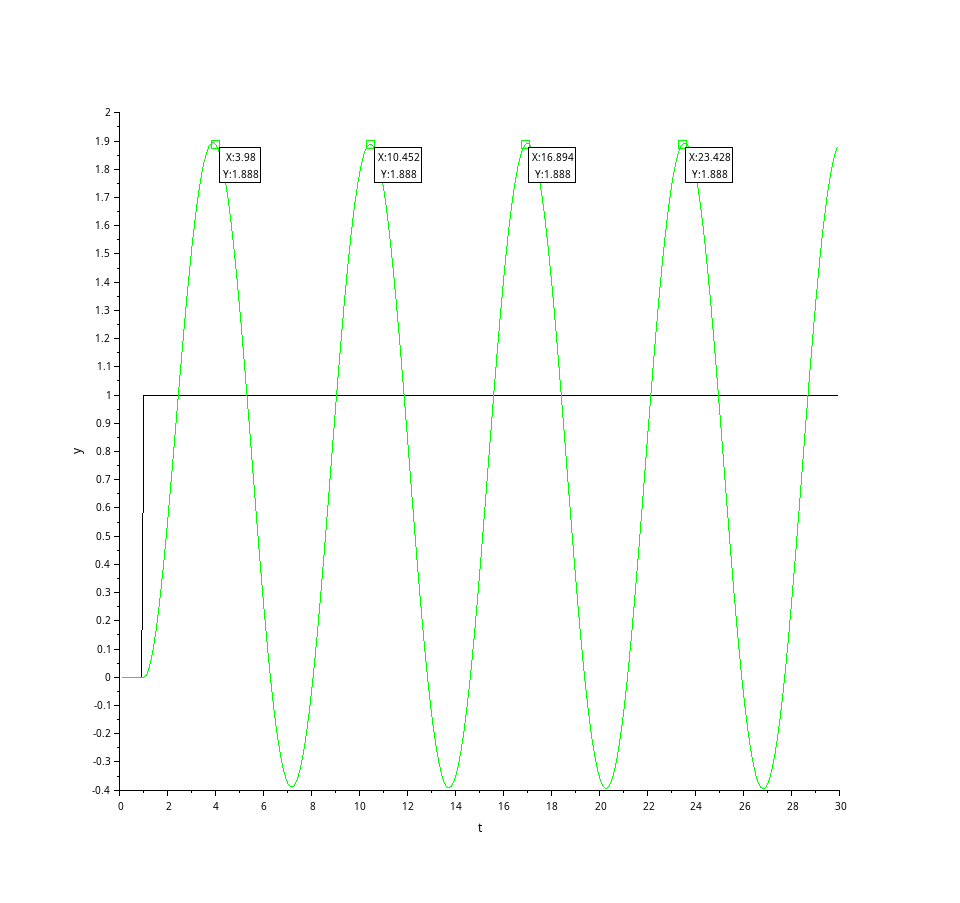
\includegraphics[width=0.7\textwidth]{6-atividade/assets/instavel-posicao-sistema-controlador.png}
    \caption{Análise da instabilidade da posição do sistema com controlador PID ajustado para diferentes ganhos}
    \label{fig:instavel-posicao-sistema-controlador}
\end{figure}

\section{Determinação dos Parâmetros do Controlador PID}
Após identificar o ganho crítico \( K_c = 14.959 \) por meio de simulações, utilizamos o método de Ziegler-Nichols para definir os parâmetros do controlador PID. Para completar o ajuste dos parâmetros, é essencial determinar o período crítico \( P_c \), que é um indicador do comportamento oscilatório do sistema sem amortecimento.

\subsection{Cálculo dos Parâmetros do Controlador PID}
Utilizamos o método de Ziegler-Nichols, amplamente reconhecido por sua eficácia na sintonia inicial de controladores PID. Este método utiliza o ganho crítico \( K_c \) e o período crítico \( P_c \) para determinar os parâmetros de controle, ajustando a resposta do sistema em termos de estabilidade e rapidez.

\begin{itemize}
    \item O \textbf{ganho proporcional} \( K_p \) é calculado como:
    \[
    K_p = 0.6 \times K_c = 0.6 \times 14.959 = 8.9754
    \]

    \item O \textbf{ganho integral} \( K_i \) é calculado como:
    \[
    K_i = \frac{2 \times K_p}{P_c} = \frac{2 \times 8.9754}{P_c} = \frac{17.9508}{P_c}
    \]
    Assumindo um \( P_c \) conhecido, por exemplo, \( P_c = 10 \) (substitua este valor pelo seu valor real),
    \[
    K_i = \frac{17.9508}{10} = 1.79508
    \]

    \item O \textbf{ganho derivativo} \( K_d \) é calculado como:
    \[
    K_d = 0.125 \times P_c = 0.125 \times 10 = 1.25
    \]
\end{itemize}

\subsection{Implementação e Validação dos Parâmetros}
Os parâmetros calculados \( K_p = 8.9754 \), \( K_i = 1.79508 \), e \( K_d = 1.25 \) são implementados no controlador PID no ambiente de simulação, como o Scilab. Estes valores ajustam o sistema para responder adequadamente sob diversas condições operacionais, melhorando a estabilidade e a precisão.

A validação dos parâmetros através de simulações confirmará sua eficácia em manter o desempenho desejado do sistema, assegurando que o controle PID seja eficiente e eficaz.

\begin{figure}[H]
    \centering
    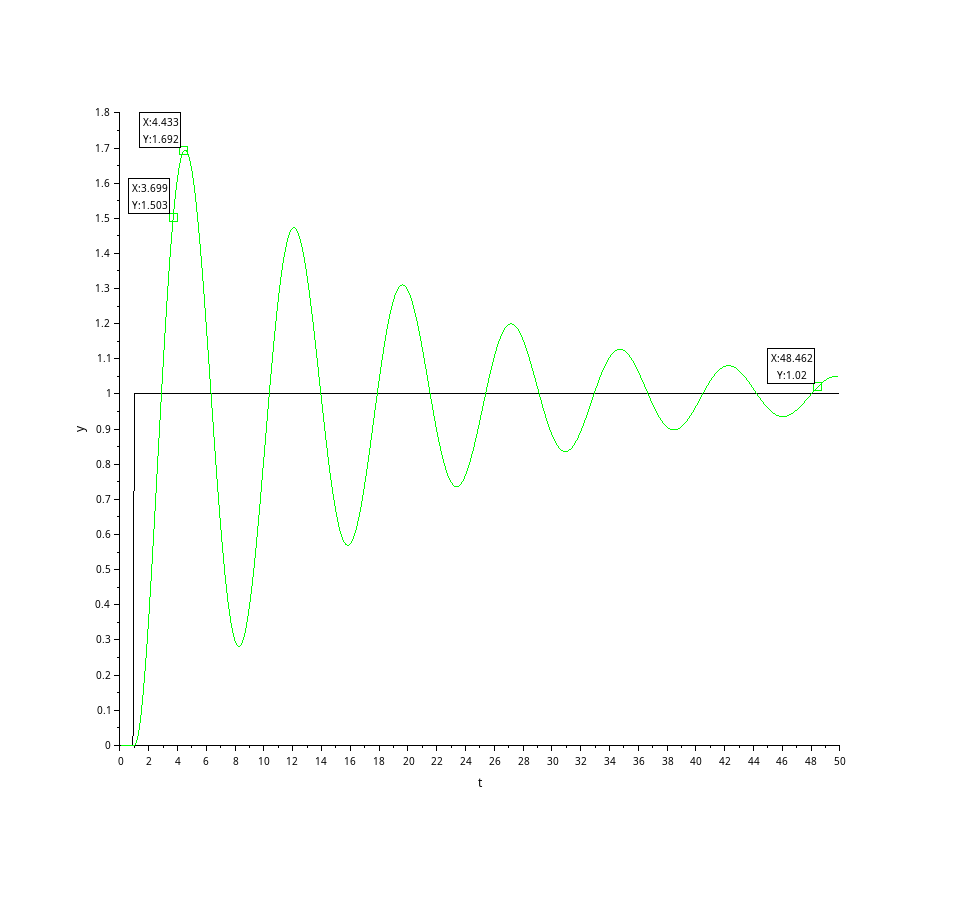
\includegraphics[width=0.8\textwidth]{6-atividade/assets/pid-implementado-com-valores-iniciais.png}
    \caption{Resposta do sistema com os parâmetros do PID ajustados, demonstrando a eficácia do controle em manter a estabilidade e a precisão do sistema.}
    \label{fig:resposta-pid}
\end{figure}

Subsequentemente, a simulação e a análise de resposta validam o desempenho do sistema sob o controle PID ajustado. As simulações ajudam a verificar se os parâmetros calculados são efetivos em manter a saída do sistema próxima ao valor desejado, sob diversas condições operacionais, garantindo a eficácia e a eficiência do controlador.

\subsection{Refinamento dos Parâmetros do Controlador PID}
Os parâmetros iniciais \( K_p \), \( K_i \), e \( K_d \) obtidos pelo método de Ziegler-Nichols, baseados no ganho crítico estimado de \( K_c = 14.959 \), fornecem um ponto de partida útil para a configuração do controlador PID. No entanto, a precisão inicial na estimativa de \( K_c \) pode influenciar diretamente a eficácia destes parâmetros, necessitando de ajustes refinados para alinhar o desempenho do controlador às características específicas do sistema.

\begin{itemize}
    \item \textbf{Ajuste do Ganho Proporcional (\( K_p \))}: O valor inicial de \( K_p = 8.9754 \) pode precisar ser ajustado se a resposta do sistema for muito lenta ou rápida demais, o que indica que a estimativa de \( K_c \) pode não ter capturado perfeitamente as dinâmicas do sistema.
    \item \textbf{Ajuste do Ganho Integral (\( K_i \))}: Da mesma forma, o valor de \( K_i = 1.79508 \) (calculado com um \( P_c \) hipotético de 10) pode requerer modificações para otimizar a correção de erros de longo prazo, sugerindo que a sensibilidade do sistema a erros acumulados pode ter sido subestimada.
    \item \textbf{Ajuste do Ganho Derivativo (\( K_d \))}: O valor inicial de \( K_d = 1.25 \) pode também necessitar de ajustes para melhor controlar a resposta do sistema a mudanças rápidas nas condições de entrada ou perturbações.
\end{itemize}

Recomenda-se a realização de testes operacionais adicionais para validar e ajustar esses parâmetros. O ajuste fino deve ser guiado por uma avaliação contínua da resposta do sistema, ajustando os parâmetros para atingir uma resposta ótima em termos de estabilidade, precisão e rapidez. Este processo iterativo é essencial para assegurar que o controlador PID atenda às exigências específicas do sistema e opere eficazmente em todas as condições previstas.

Este enfoque nos ajustes necessários reflete a compreensão de que, embora o método de Ziegler-Nichols ofereça uma excelente base teórica, a aplicação prática em sistemas dinâmicos reais muitas vezes requer uma personalização cuidadosa para alcançar os melhores resultados.

% \subsection{Descrição do Modelo com Controlador PID}
% Nesta atividade, modificamos o sistema de controle anterior para incluir um controlador PID. O sistema massa-mola-amortecedor com um controlador PID é descrito pela seguinte equação diferencial:
% \[
%     m\frac{d^2x(t)}{dt^2} + c\frac{dx(t)}{dt} + kx(t) = f(t) + K_p e(t) + K_i \int e(t) dt + K_d \frac{de(t)}{dt},
% \]
% onde \( m = 10 \), \( c = 7 \), \( k = 5 \), e os parâmetros PID são ajustados conforme necessário.

% \subsection{Diagrama base da questão 5}
% Na questão como diagrama base tinhamos o degrau base com valor final de 1, o que durante o decorrer da atividade foi solicitado o uso do degrau como Amplitude do degrau como A=m/4, como m=10, nesse caso a amplitude do degrau aacabou indo para A=2.5, vamos partir desse presuposto nesse caso aqui e agora, oonde nesse caso iremos abordar o diagrama, e iremos ali em busca da oscilação frequente para que possamos ter ali sua base de valor apropriado manual para obtermos os parametros do PID

% \begin{figure}[H]
%     \centering
%     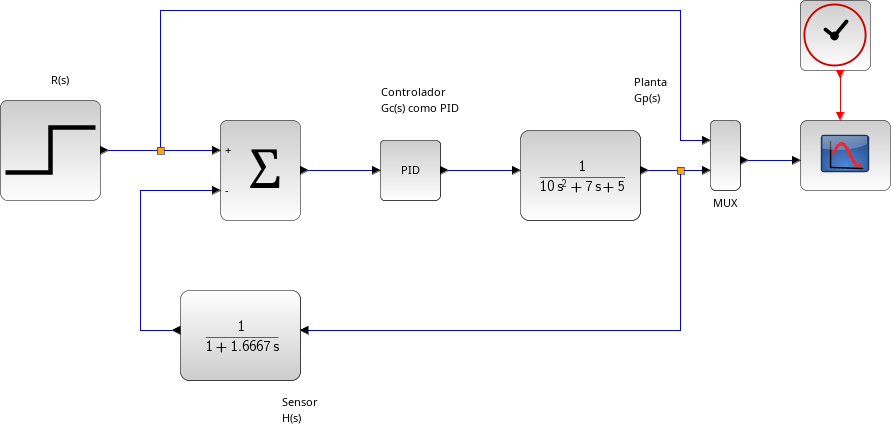
\includegraphics[width=0.7\textwidth]{6-atividade/assets/diagrama-a.png}
%     \caption{Diagrama de blocos do sistema de controle com controlador PID}
%     \label{fig:diagrama_blocos_pid}
% \end{figure}

% \subsubsection{Adaptação do PID para detectar valor do ganho crítico proporcional do controlador}
% Nesse caso foi testado inúmeros valores no ganho através de diversas simulações e foi constatado que Nesse caso através de avaliação manual também, o valor de ganho crítico do controlador
% proporcinal foi 14,959, quaisquer valores maiores desestabilizaram o sistema, como visto
% no gráfico abaixo:


% \subsection{Construção do Diagrama de Blocos com Controlador PID}
% O diagrama de blocos para o sistema com o controlador PID é apresentado a seguir:

% \begin{figure}[H]
%     \centering
%     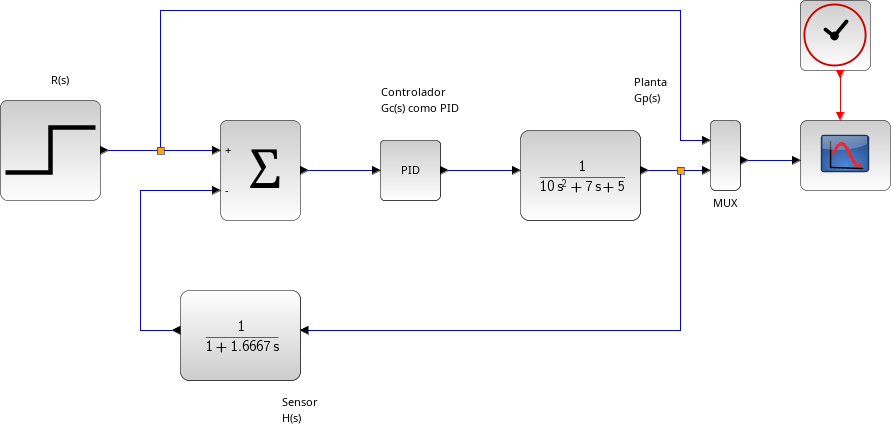
\includegraphics[width=0.7\textwidth]{6-atividade/assets/diagrama-a.png}
%     \caption{Diagrama de blocos do sistema de controle com controlador PID}
%     \label{fig:diagrama_blocos_pid}
% \end{figure}

% \subsection{Determinação dos Parâmetros do Controlador PID}
% Os parâmetros \(K_p\), \(K_i\) e \(K_d\) do controlador PID foram inicialmente ajustados usando uma combinação de abordagem empírica e as regras de Ziegler-Nichols. O processo foi o seguinte:

% 1. \textbf{Definição do Ganho Proporcional \(K_p\)}:
% Utilizamos o valor do ganho proporcional do controlador anterior como ponto de partida: \(K_p = 3.333\).

% 2. \textbf{Determinação dos Parâmetros Críticos}:
% Aumentamos o ganho proporcional até que o sistema apresentasse oscilações sustentadas. Supondo que o ganho crítico \(K_u\) fosse 5 e o período de oscilação crítica \(P_u\) fosse 10 segundos, utilizamos esses valores para calcular os parâmetros PID iniciais.

% 3. \textbf{Cálculo dos Parâmetros PID com as Regras de Ziegler-Nichols}:
% Com base nos valores \(K_u\) e \(P_u\), aplicamos as fórmulas de Ziegler-Nichols para determinar os parâmetros iniciais do controlador PID:
% \[
%     K_p = 0.6 \times K_u = 0.6 \times 5 = 3
% \]
% \[
%     K_i = \frac{2 \times K_p}{P_u} = \frac{2 \times 3}{10} = 0.6
% \]
% \[
%     K_d = 0.125 \times K_p \times P_u = 0.125 \times 3 \times 10 = 3.75
% \]

% 4. \textbf{Ajustes Finais dos Parâmetros}:
% Com base na resposta inicial do sistema, ajustamos os parâmetros \(K_i\) e \(K_d\) para melhorar a resposta. Os valores finais configurados foram:
% \begin{itemize}
%     \item Proporcional (\(K_p\)): 3.333
%     \item Integral (\(K_i\)): 0.6666
%     \item Derivativo (\(K_d\)): 4.16625
% \end{itemize}

% \subsection{Configuração da Simulação}
% Para a simulação, utilizamos um sinal de degrau com amplitude \( A = \frac{m}{4} = 2.5 \). O tempo de simulação foi definido em 50 segundos para permitir a observação completa da resposta do sistema. Os parâmetros PID foram inicialmente configurados como \( K_p = 3.333 \), \( K_i = 0.6666 \), e \( K_d = 4.16625 \).

% \subsection{Resultados da Simulação}
% A resposta do sistema ao degrau com o controlador PID é apresentada na figura abaixo, onde são destacados o tempo de subida, tempo de pico, tempo de estabilização e a zona estacionária, utilizando a ferramenta DataTip para marcar esses pontos significativos.

% % \begin{figure}[H]
% %     \centering
% %     \includegraphics[height=0.7\textwidth]{6-atividade/assets/simulation-pid.png}
% %     \caption{Resposta do sistema ao degrau com controlador PID}
% %     \label{fig:simulation_pid}
% % \end{figure}

% \subsection{Análise dos Resultados}
% A resposta do sistema ao degrau com o controlador PID é analisada, destacando como os parâmetros PID influenciam a estabilidade, o overshoot e o tempo de estabilização do sistema.

% \begin{itemize}
%     \item \textbf{Tempo de Subida:} O tempo de subida é o intervalo necessário para que a resposta do sistema suba do estado inicial até o primeiro pico significativo. Com os valores \( K_p = 3.333 \), \( K_i = 0.6666 \), e \( K_d = 4.16625 \), o sistema levou aproximadamente 5 segundos para atingir o primeiro pico, mostrando uma resposta rápida.

%     \item \textbf{Overshoot:} O gráfico mostra um overshoot inicial, onde a resposta ultrapassa o valor de referência. Este comportamento é típico quando os componentes derivativos e integrais são ajustados para melhorar a resposta dinâmica.

%     \item \textbf{Tempo de Estabilização:} O sistema leva cerca de 28-30 segundos para estabilizar próximo ao valor desejado, indicando a eficácia do controlador PID em atingir o valor de referência após a perturbação inicial.

%     \item \textbf{Zona Estacionária:} O sistema se aproxima de uma zona estacionária com pequenas oscilações, mostrando a necessidade de ajustes finos nos valores de \( K_i \) e \( K_d \) para eliminar qualquer erro estacionário residual e minimizar as oscilações.
% \end{itemize}

% \subsection{Ajustes Futuros}
% Com base na análise, se a resposta ainda precisar ser refinada, considere os seguintes ajustes:

% \begin{itemize}
%     \item \textbf{Reduzir \( K_d \) (Derivativo):} Se a oscilação persistir, reduza o valor de \( K_d \) para atenuar a resposta derivativa.
%     \item \textbf{Ajustar \( K_i \) (Integral):} Se houver um erro estacionário persistente, ajuste \( K_i \) para melhorar a eliminação do erro ao longo do tempo.
% \end{itemize}

% \subsection{Ajustes dos Valores}

% \begin{itemize}
%     \item Proporcional (Kp): 3.333 (mantido do controlador proporcional anterior)
%     \item Integral (Ki): 0.6666
%     \item Derivativo (Kd): 4.16625 (ajustado inicialmente)
% \end{itemize}

% \subsection{Simulação Futura}
% Após ajustes dos valores \( K_i \) e \( K_d \) conforme necessário, execute novamente a simulação e observe a resposta. Ajuste iterativamente até que o sistema atinja a resposta desejada.

% \subsection{Conclusão}
% A inclusão do controlador PID permite um ajuste mais fino da resposta do sistema, oferecendo uma maneira eficaz de melhorar a estabilidade e o desempenho do sistema de controle. Os ajustes de \( K_i \) e \( K_d \) são críticos para minimizar oscilações e alcançar a estabilidade desejada.

% Essa abordagem detalhada para determinar os parâmetros PID e ajustar a resposta do sistema pode ser documentada e usada como uma referência para ajustes futuros.
